\documentclass[12pt, dvipsnames, svgnames, x11names,]{article}

\usepackage{xcolor}
% URLs and hyperlinks ---------------------------------------
\usepackage{hyperref}
\hypersetup{
	colorlinks=true,
	linkcolor=NavyBlue,
	filecolor=magenta,      
	urlcolor=blue,
}
\usepackage{xurl}
%---------------------------------------------------
\usepackage[inline]{enumitem}
\usepackage{graphicx}
\usepackage{multirow}
\usepackage{float}
\renewcommand{\arraystretch}{1.40}

% adjust a verrrrry big table -------------------------------
\usepackage{adjustbox}
% -----------------------------------------------------------

\usepackage{array}
% center the p columns and m --------------------------------------------------------------
\newcolumntype{P}[1]{>{\centering\arraybackslash}p{#1}}
\newcolumntype{M}[1]{>{\centering\arraybackslash}m{#1}}
% -------------------------------------------------------------------------------------------------------------

% price
\usepackage{marvosym}
% ----------

\usepackage{xepersian}
\settextfont{Yas}
\setdigitfont{Yas}

\begin{document}
	\begin{titlepage}
		\centering
		\vspace{1cm}
		{\Huge {\textbf{\lr{FOL - Tour offer}}}\par}
		\vspace{15mm}
		\vspace{16mm}
		
\includegraphics[width=12cm]{images/01} \par
		\vfill \par	\vfill
		\vspace{16mm}
		{\normalsize	سیدمحمدحسین هاشمی  4022363143 \par}
		
		\vspace{1cm}
		{\large دی ۱۴۰۲\par}
	\end{titlepage}
	\tableofcontents
	
	\section{\lr{TODO 1} - آماده سازی پایگاه دانش}
		
		\subsection{شهرها و امکانات با روش \lr{flat fact} وارد پایگاه دانش می‌شود .}
			\begin{center}
				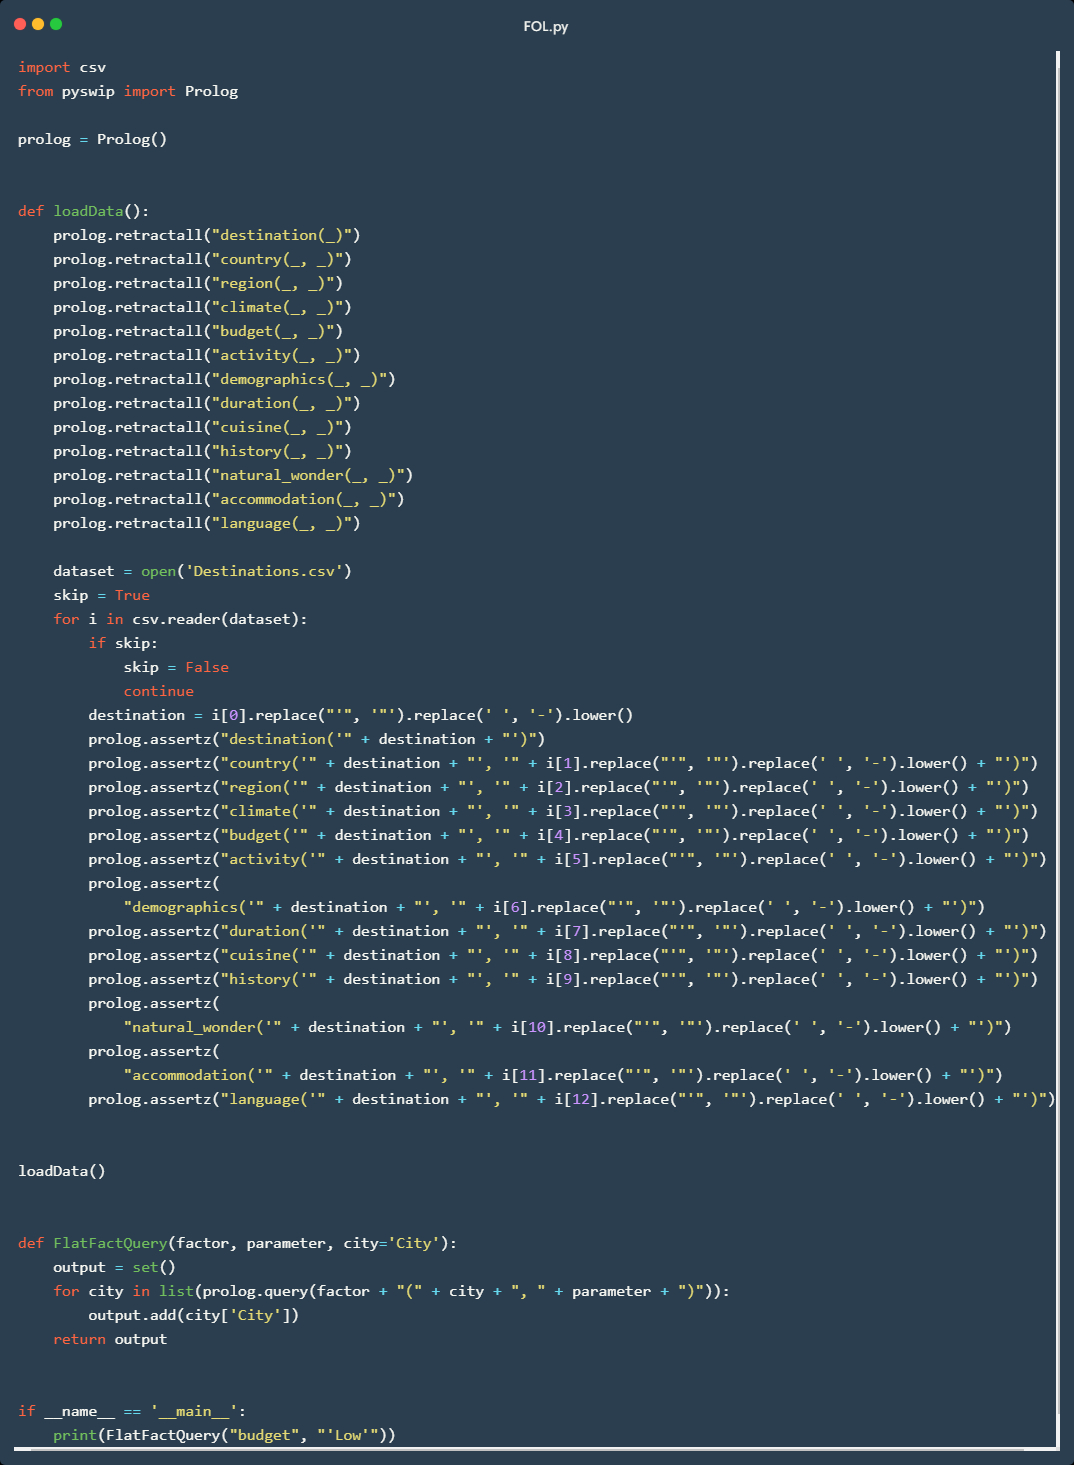
\includegraphics[width=12cm]{images/02}
			\end{center}
			
		\subsection{اتصالات شهرها 3 مرحله بررسی و با ویژگی \lr{connected} مورد بررسی هستند.}
			\begin{center}
				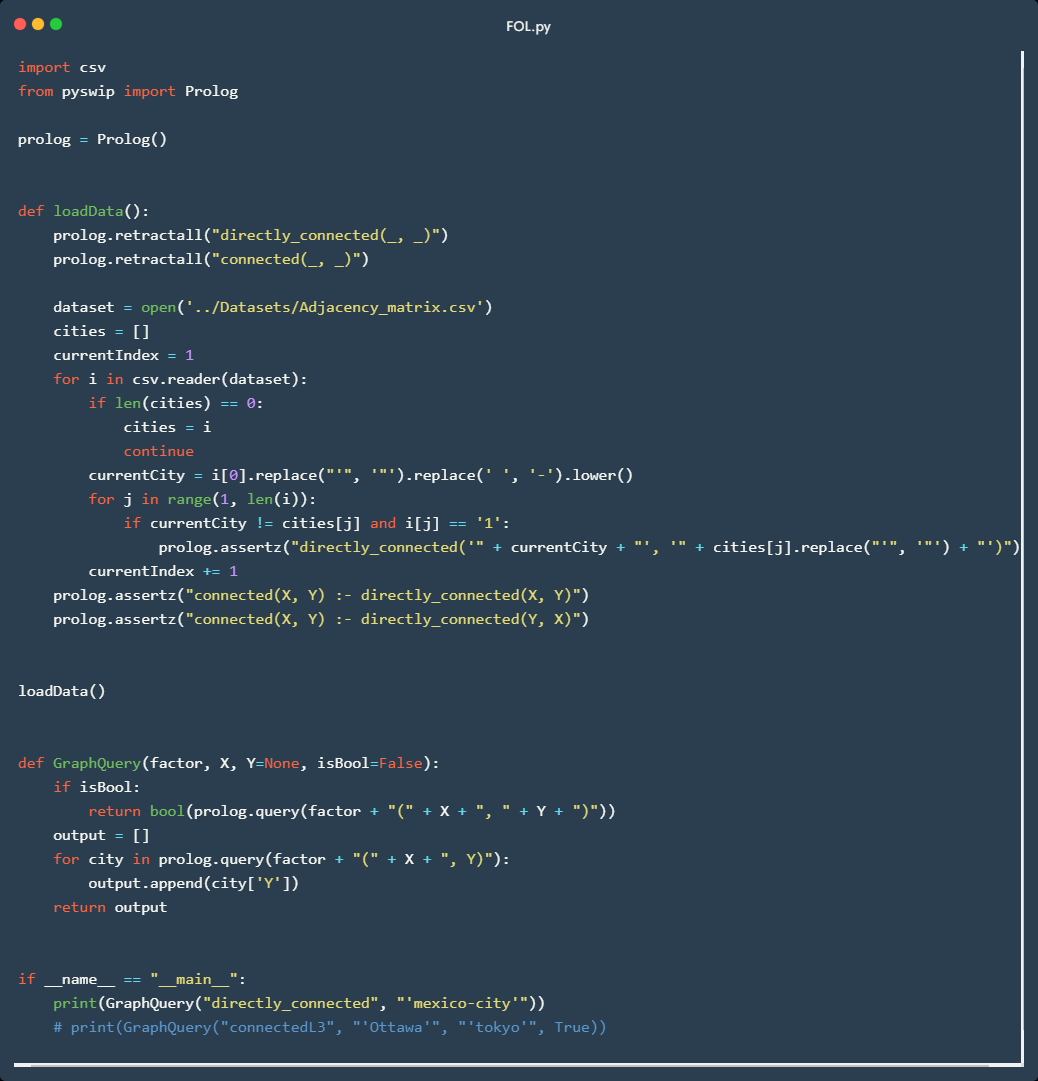
\includegraphics[width=12cm]{images/03}
			\end{center}
			
	
	\section{\lr{TODO 2} - یافتن کلیدهای انواع ویژگی‌ها}
		\begin{center}
			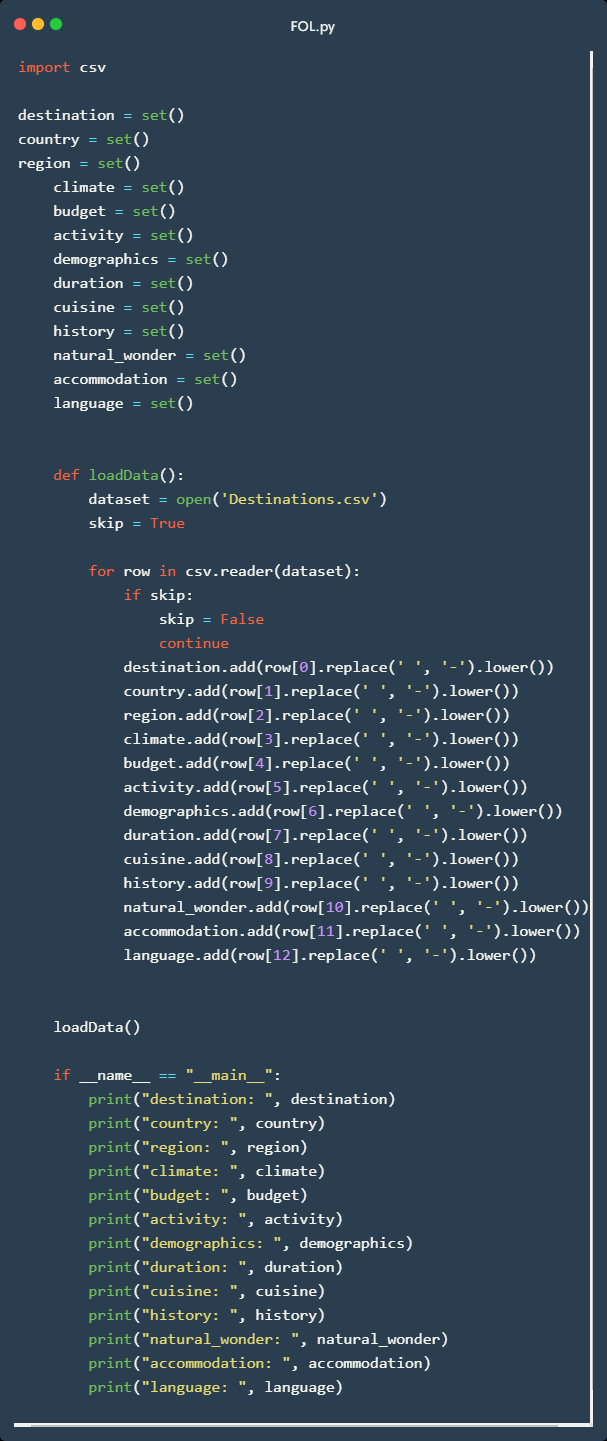
\includegraphics[width=7cm]{images/04}
		\end{center}
	
	\section{\lr{TODO 3} - دریافت کلمات کلیدی از جمله ورودی}
		\begin{center}
			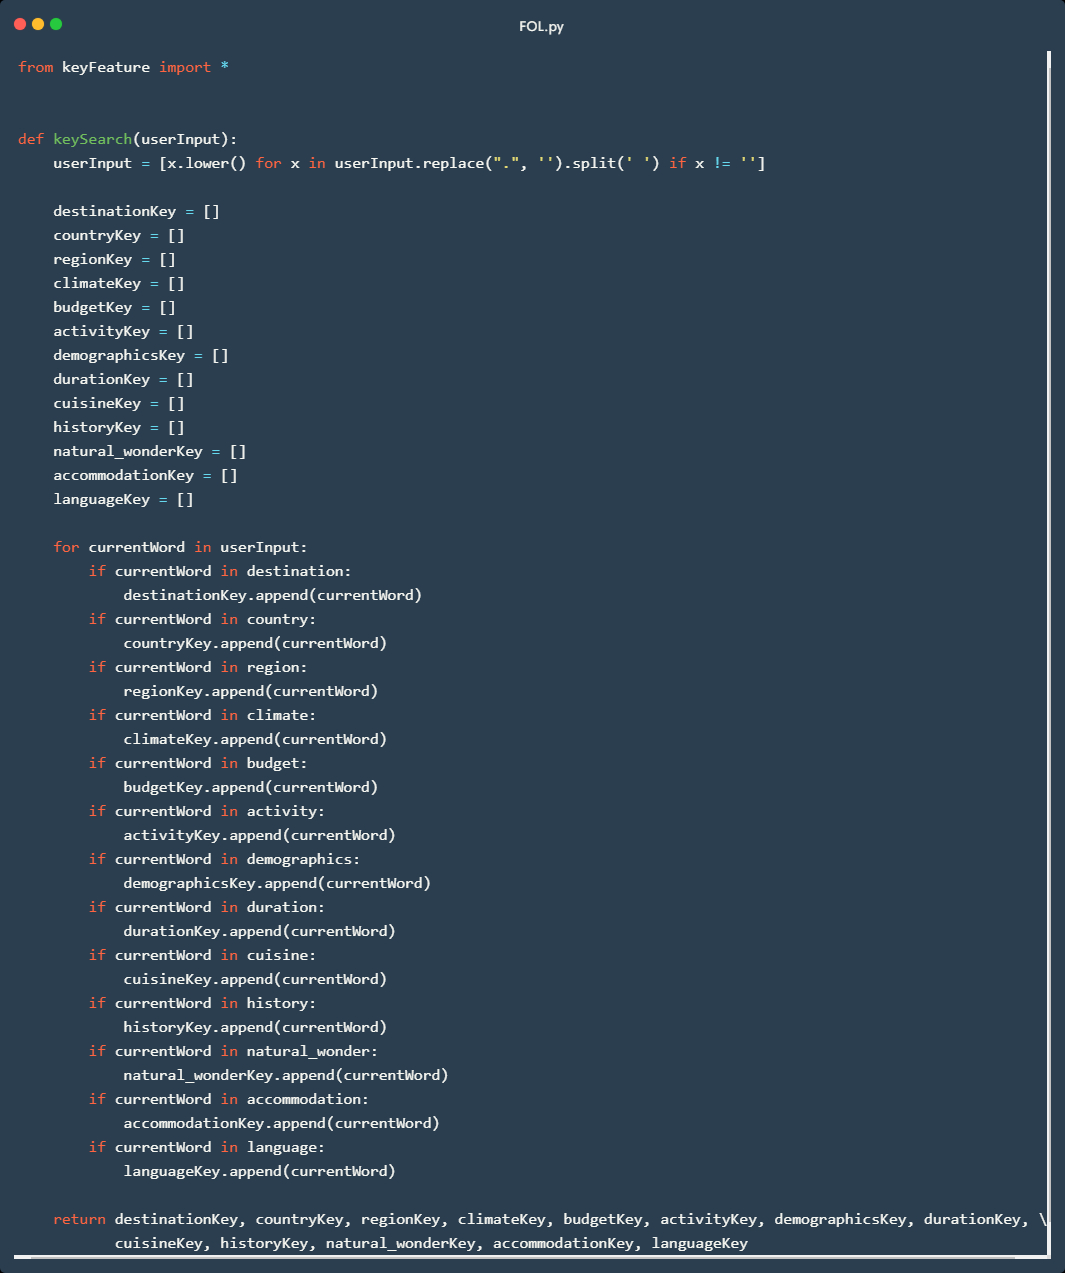
\includegraphics[width=12cm]{images/05}
		\end{center}
	
	\section{\lr{TODO 4} - دریافت لیست شهرها بر اساس ویژگی‌ها}
		\begin{center}
			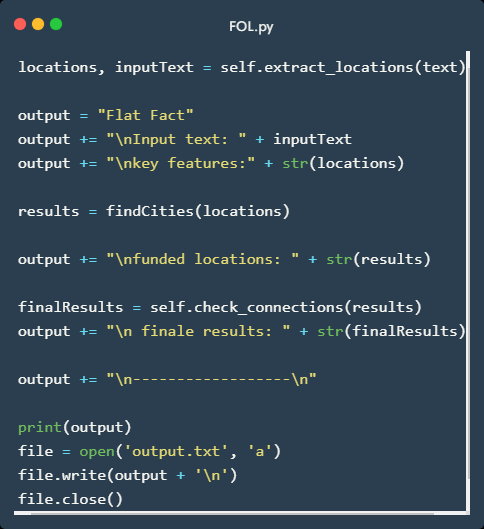
\includegraphics[width=8cm]{images/06}
		\end{center}
		{\normalsize در این قسمت تابع \lr{findCities} فراخوانی و همچنین محتوای فایل \lr{outputs} آماده می‌شود.} \par
		\begin{center}
			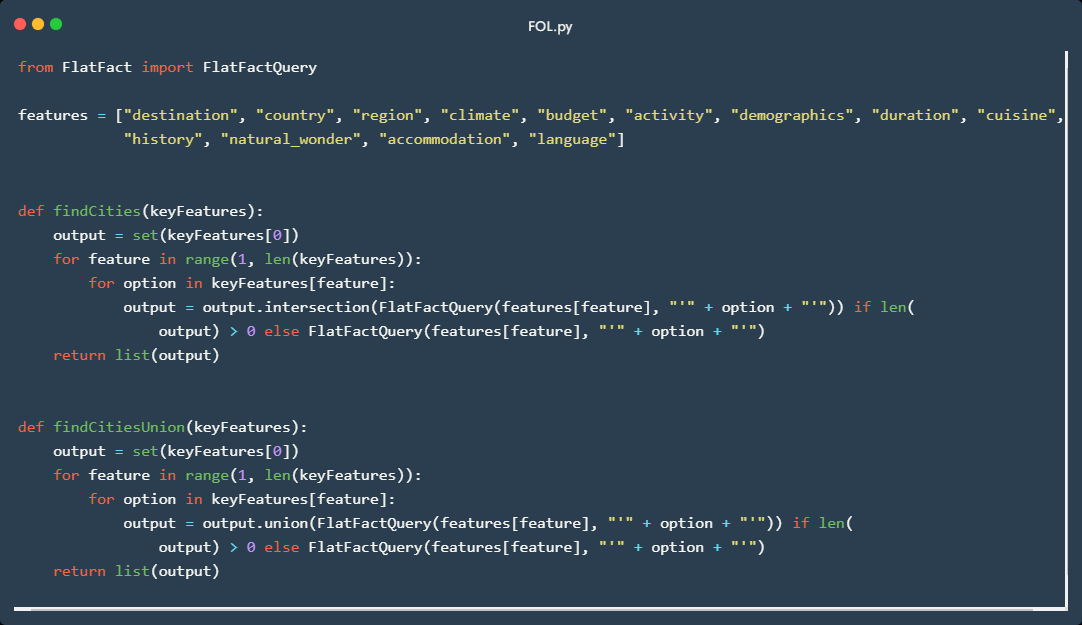
\includegraphics[width=13cm]{images/07}
		\end{center}
		{\normalsize این تابع با فراخوانی \lr{FlatFactQuery} و اشتراک گرفتن خروجی آن با خروجی سایر ویژگی‌ها شهرهای مطابق را پیدا می‌‌کند.}
	
	\section{\lr{TODO 5} - بررسی اتصال شهرها}
				\begin{center}
			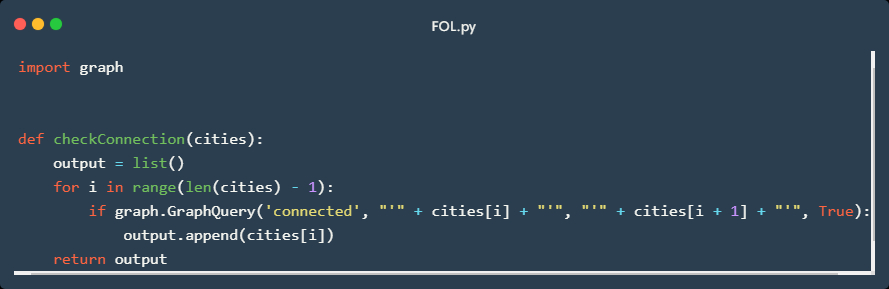
\includegraphics[width=8cm]{images/08}
		\end{center}
		{\normalsize این تابع براساس پایگاه دانش شهرهای متصل به یکدیگر را برمی‌گرداند.}
	
	\section{\lr{TODO 6} - بررسی تعداد و نمایش خروجی}
		\begin{center}
			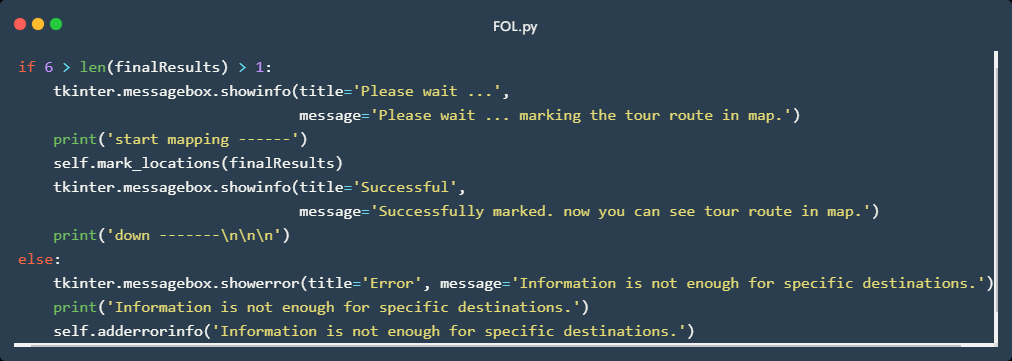
\includegraphics[width=13cm]{images/09}
		\end{center}
		{\normalsize در این قسمت در صورتی که تعداد شهرها بین 1 تا 6 شهر باشد آن را روی نقشه چاپ وگرنه خطا برمی‌گرداند.}
		
	
	
	
\end{document}